\chapter{Control Schemes}
\textit{In this chapter the purpose is to describe the design of the controllers for the satellite. First, a desaturation controller is designed for distributing the torque between the actuators. A second controller is the hybrid attitude one, which is capable of taking care of the tumble of the satellite. Next, based on previous work, two types of attitude controllers are designed. For making a comparison between a linear controller and non-linear one, a state feedback controller and a sliding mode controller are presented.}

The proposed control scheme presented in figure \ref{fig:mainLoop} has a hierarchical, modular structure. The main attitude controller outputs a torque reference for the actuators, which is then distributed by lower level controllers. This means that the attitude controller can be swapped without having to modify the lower level controllers. The desaturation controller distributes the torque between the reaction wheels and magnetorquers. The reaction wheel subsystem executes local fault detection and fault isolation. It receives a 3 dimensional torque demand and distributes it between the individual reaction wheel motors. The reaction wheels subsystem checks fault residual signals and adjusts torque distribution between reaction wheels accordingly. 
\begin{figure}[h!]
	\centering 
	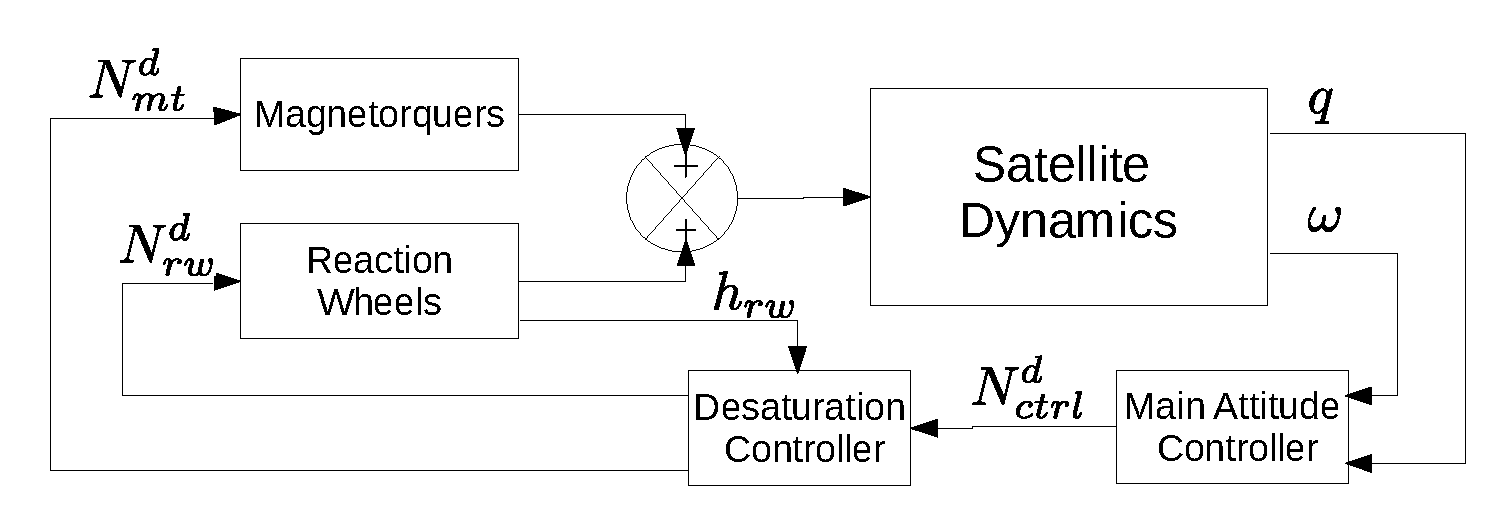
\includegraphics[width=160mm]{figures/mainLoop.pdf}	
	\caption{Main Control Loop.}
	\label{fig:mainLoop}
\end{figure}

\todo{add reference omega and q to figure}
\todo{evaluation of station tracking precision - should be within $1\deg$. Compare different reaction wheel configurations}

		\begin{equation}
		\underline{I}_{s}\vec{\dot{\omega}} + \underline{\omega}^\times\underline{I}_{s}\vec{\omega} = -\vec{\dot{h}}_{rw} -  \underline{\omega}^\times \vec{{h}}_{rw} + \vec{N_{mt}}  + \vec{N_{dist}} =  -  \underline{\omega}^\times \vec{{h}}_{rw} + \vec{N_{rw}} + \vec{N_{mt}}  + \vec{N_{dist}} 
		\end{equation}
		
		Compensation for $\underline{\omega}^\times \vec{{h}}_{rw}$ for torque demand inputs \todo{compensation} 

\section{Desaturation}

The reaction wheel DC motors and bearings have a limited angular velocity range they can operate in. When the velocity reaches the limit, the motor can no longer accelerate the wheel further in one direction, thus reducing controllability. To avoid this, the wheel velocity should be kept near zero. Usually the speed is above zero to avoid static friction in the bearings. Decreasing the reaction wheel speed by transferring its angular momentum is called desaturation.

Reaction wheels are used to control the attitude of the satellite by transferring its angular momentum. Transferring the angular momentum back to the satellite body would be counterproductive, it should be discarded in a different way. Magnetorquers are ideal for desaturation since they can interact with the earth's magnetic field and are able to transfer angular momentum of the satellite body to earth. Since the earth's magnetic field is quite weak, the torque produced by magnetorquers are small compared to the torque of the reaction wheels. Reaction wheels can be used for fast attitude control while magnetorquers are good for gradually desaturating the reaction wheels. The angular momentum transfer happens through the satellite's body, but with the right control scheme the desaturation can be  completely decoupled from attitude control.

Trégouët et al. \cite{DesatTregouet} developed a cascaded control method for reaction wheel desaturation. The method is a revised version of the so-called cross-product control law. It changes the magnetorquers' magnetic field based on the difference between the angular momentum of the reaction wheels and their reference angular momentum.

\begin{equation}
\vec{\tau_m} = -\frac{\underline{\tilde{b}}^\times(t)}{|\vec{\tilde{b}}(t) |^2} k_p\left(\vec{h_{rw}} - \vec{h_{ref}} \right)
\end{equation}

where  \todo{add the notations to nomenclature}

Momentum dumping and attitude control can potentially be opposing goals, since attitude control changes the reaction wheel velocity to produce the required torque, while the desaturator tries to keep the angular velocity close to the reference. The quasi-cascaded structure of the desaturation control law includes the magnetorquer as the upper subsystem which outputs the rate of change of the total angular momentum of the system \ref{fig:CascadeDesat}. The lower subsystem includes the attitude dynamics and the reaction wheel controller. The problem is that there's a feedback involved from the lower subsystem to the upper one, making $\dot{h}_t$ dependent on the attitude parameters. This means that desaturating the wheels can affect the attitude control loop. Since attitude control is more crucial than desaturation, the reverse would be desirable.  By reversing the ordering of the cascade, the interference can be eliminated. It is done by applying input allocation, i.e. "suitably assigning the low level actuators' input, based on a higher level control effort requested by the control system" \cite{JOHANSEN20131087}. From the point of view of the desaturation controller, the control goal is to keep the reaction wheels' angular velocity as close to the reference velocity as possible. Since the desaturation control is decoupled from attitude control, it can achieve its desaturation control goal regardless of the attitude control law.




\begin{figure}[h]
	\centering
	\begin{tabular}{@{}c@{\hspace{.5cm}}c@{}}
		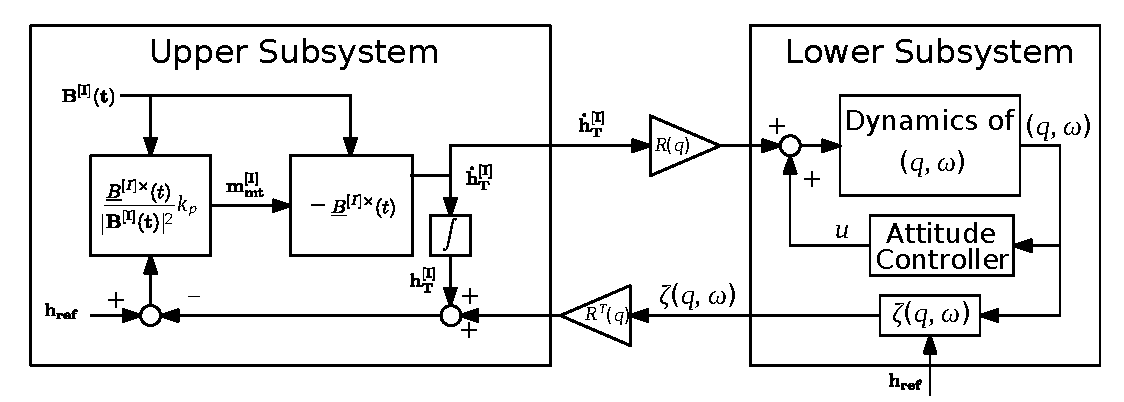
\includegraphics[page=1,width=1\textwidth]{quasiCascadeDesat.pdf}
	\end{tabular}
	\caption{Quasi cascaded desaturation control scheme \cite[Fig. 2.]{DesatTregouet}}
	\label{fig:quasiCascadeDesat}
\end{figure}

According to equation \todo{ref eq in modelling}

\begin{equation}
\underline{I}_{s}\vec{\dot{\omega}} + \underline{\omega}^\times\underline{I}_{s}\vec{\omega} = -\vec{\dot{h}}_{rw} -  \underline{\omega}^\times \vec{{h}}_{rw} + \vec{N_{mt}}  + \vec{N_{dist}} = \vec{u} 
\end{equation}

\begin{equation}
\vec{\tau_m}^{[I]} = -\frac{\underline{\tilde{b}}^\times(t)}{|\vec{\tilde{b}}(t) |^2} k_p\left(\vec{h_{rw}}^{[I]} - \underline{R}^T(\vec{q})\vec{h_{ref}} \right)
\end{equation}

\todo{make it a system of equations}

%\begin{equation}
%\dot{x}_c = 0, (\vec{q},\vec{\omega},x_c) \in C\
%\end{equation}
%
%\begin{equation}
%x_c^+ = -x_c, (\vec{q},\vec{\omega},x_c) \in D\
%\end{equation}
%
%\begin{equation}
%\vec{u} = -c x_c \epsilon -K_\omega \vec{\omega}
%\end{equation}
%
%\begin{equation}
%C:= \left\lbrace (\vec{q},\vec{\omega},x_c) \in \mathbb{S}^3 \times \mathbb{R}^3 \times \left\lbrace -1,1 \right\rbrace : x_c\eta \geq -\delta \right\rbrace 
%\end{equation}
%
%\begin{equation}
%D:= \left\lbrace (\vec{q},\vec{\omega},x_c) \in \mathbb{S}^3 \times \mathbb{R}^3 \times \left\lbrace -1,1 \right\rbrace : x_c\eta \leq -\delta \right\rbrace 
%\end{equation}

as shown in \ref{eq:finaleq}
\begin{flalign}
\vec{ ^s_i\dot q(t)}  = \dfrac{1}{2} \underline \Omega \  \vec{^s_i q(t)}
\end{flalign} 

\[
\begin{array}{l}

\dot{x}_c = 0, (\vec{q},\vec{\omega},x_c) \in C\ \\ 
x_c^+ = -x_c, (\vec{q},\vec{\omega},x_c) \in D\ \\ 
\vec{u} = -c x_c \epsilon -K_\omega \vec{\omega} \\
C:= \left\lbrace (\vec{q},\vec{\omega},x_c) \in \mathbb{S}^3 \times \mathbb{R}^3 \times \left\lbrace -1,1 \right\rbrace : x_c\eta \geq -\delta \right\rbrace  \\

D:= \left\lbrace (\vec{q},\vec{\omega},x_c) \in \mathbb{S}^3 \times \mathbb{R}^3 \times \left\lbrace -1,1 \right\rbrace : x_c\eta \leq -\delta \right\rbrace 
\end{array}
\]

\todo{this attitude controller should be down as one of the possible attitude controllers - "Satellite angular momentum removal utilizing the earth’s magnetic field" article}

\begin{figure}[h]
	\centering
	\begin{tabular}{@{}c@{\hspace{.5cm}}c@{}}
		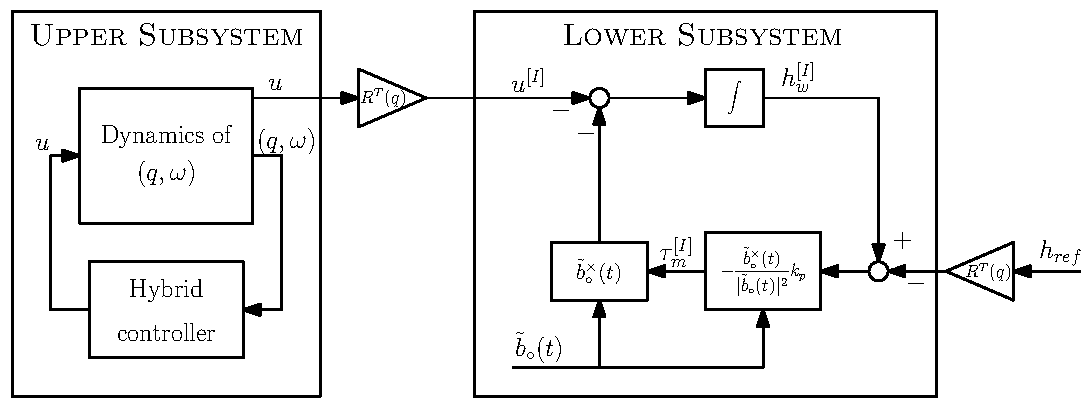
\includegraphics[page=1,width=1\textwidth]{cascadeDesat.pdf}
	\end{tabular}
	\caption{Cascaded desaturation control scheme  \cite[Fig. 4.]{DesatTregouet}}
	\label{fig:CascadeDesat}
\end{figure}

The derived equations that can be implemented in simulation:

\begin{equation}
\vec{\dot{\omega}} = \underline{I}_{s}^{-1}\left( \vec{u} -  \underline{\omega}^\times\underline{I}_{s}\vec{\omega}  \right) 
\end{equation}

\begin{equation}
\vec{\dot{h}}_{rw} =  -  \underline{\omega}^\times \vec{{h}}_{rw} + \vec{N_{mt}}  + \vec{N_{dist}} - \vec{u} 
\end{equation}

\todo{body-fixed frame
	Static input allocation
	global asymptotic stability}

\cite{DesatYang}
\section{Main Attitude Controller}
\label{sec:mainCont}

\textit{Previously the main attitude controller was treated as a black box. The current and subsequent sections discuss several satellite attitude controllers.}

\subsection{Hybrid Attitude Controller}

Dynamic discontinuous hybrid controller, global asymptotic stability, local exponential stability, state feedback for $\omega$ and $q$. Capable of detumbling. \cite{globalAttController}

There are different ways to describe the rotation of a 3D object. One of them is by using Euler sequences consisting of 3 rotational values. Euler rotation sequences can use combinations of roll, pitch and yaw. There's an inherent problem with Euler rotation, that makes controlling Euler rotation based models an issue, i.e. they are susceptible to singularities. Certain orientations might have an infinite amount of corresponding Euler angles. This can arise when the rotations are made in such a way that some rotation axes align with each other. This issue is commonly known as the gimbal lock. The result of a gimbal lock is that given an attitude, the  cannot be unambiguously deducted, unless extra constraints are introduced.

Quaternion based rotation representation are more appropriate for control. Quaternions are not susceptible to singularities. The only problem with quaternion representation is the so-called double coverage, i.e. rotation by $-\vec{q}$ represents the same rotation as rotation by $-\vec{q}$. This becomes obvious from the rotation equation \ref{eq:doubleCover}.

\begin{equation}
\label{eq:doubleCover}
\vec{q} \vec{v} \vec{q}^{-1} = 	(\vec{-q}) \vec{v} (\vec{-q}^{-1})
\end{equation} 

The attitude control goal can be described as tracking the orientation demand $\vec{q}$. According to \cite{globalAttController}, it is impossible to design a globally stabilizing quaternion based state feedback that is robust to measurement noise. The quaternion-based robust hysteretic feedback controller which is capable of globally asymptotically stabilizing a rigid body is described subsequently, according to \cite{globalAttController}. It can be considered as a more robust extension of classical state feedback controller.


The dynamics of a rigid body is described in equation \ref{eq:dynSimple1}. For clarity of the control method, disturbance torques are emitted from the equation. Since the control system compensates for the gyroscopic term, it is omitted as well from the discussion .

\begin{equation}
\label{eq:dynSimple1}
\underline{I}_s \vec{\dot{\omega}} = \underline{\omega}^\times \underline{I}_s \vec{\omega} + \vec{N_{ctrl}}
\end{equation}

The control goal can be clearly described with rotation matrices. Rotation matrices use 9 variables to describe a rotation, but they have the advantage of being non-ambiguous. The rotation error can be described using equation \ref{eq:rotationError}. 

\begin{equation}
\label{eq:rotationError}
\underline{R}(\vec{q^e}) = \underline{R}(\vec{q^d})^T \underline{R}(\vec{q})
\end{equation}

The goal is to align $\underline{R}(\vec{q})$ with $\underline{R}(\vec{q^d})$ orientation demand. If that demand is satisfied, $\underline{{R}}(\vec{q^e})$ orientation error becomes $\underline{I}$ identity matrix. In quaternion representation, this goal corresponds to having having a unit quaternion with the scalar element being $\pm 1$, according to equation \ref{eq:stabilityQuat}. 

\begin{equation}
\label{eq:stabilityQuat}
\underline{R}(\vec{q^e}) = \underline{R}(\vec{q^e}) = \underline{1} \xrightarrow{equivalent} \vec{q^e}  = \pm	\begin{bmatrix}
0 \\
0 \\
0 \\
1
\end{bmatrix} 	
\end{equation}

Because of the double coverage property of quaternions, stabilizing an attitude, stabilization has to be done on a two equilibrium points corresponding to $\vec{q^e}$ in equation \ref{eq:stabilityQuat}. If a feedback controller is used in the form of $\vec{N_{ctrl}} = f(\vec{q^e})$, $\vec{q^e}$ and $-\vec{q^e}$ might result in different torque demand, even though they both represent the same rotation. The hybrid controller addresses this issue. According to \cite{globalAttController}, robust and global stabilization on this set is impossible to achieve using non-hybrid discontinuous state feedback in the presence of sensor noise. The paper proposes a hybrid, discontinuous, hysteretic, robust, gloablly asymptotically stabilizing attitude control method instead. A system is considered a hybrid system in the subsequent discussion if the state changes can vary between being continuous or discrete.

The state changes are controlled by the following rules. Controller state storing information about which of the double covering quaternions should be tracked is introduced as $x_c \in  \left\lbrace -1,1 \right\rbrace $. $x_c$ decides which of the two double covering quaternions should be tracked. If $x_c = signum(q_4)$ rule is followed, the controller becomes sensitive to measurement noise. To avoid that, a hysteresis introduced, with an adjustable $\delta  \in (0,1)$ hysteresis threshold parameter. The rule for choosing between discrete or continuous control mode is presented in equation \ref{eq:contDiscont}.

\begin{align}
\label{eq:contDiscont}
C:= \left\lbrace (\vec{q},\vec{\omega},x_c) \in \mathbb{S}^3 \times \mathbb{R}^3 \times \left\lbrace -1,1 \right\rbrace : x_c q_4 \geq -\delta \right\rbrace  \\
\nonumber D:= \left\lbrace (\vec{q},\vec{\omega},x_c) \in \mathbb{S}^3 \times \mathbb{R}^3 \times \left\lbrace -1,1 \right\rbrace : x_cq_4 \leq -\delta \right\rbrace 
\end{align}

If $(\vec{q},\vec{\omega},x_c) \in C$, i.e. the controller is running in continuous mode, the governing equations are according to equation \ref{eq:globalCont}. When $(\vec{q},\vec{\omega},x_c) \in D$, $x_c$ controller state swaps sign instantaneously. Because of the $\delta$ thresholding, two swaps don't happen in infinitesimally small time.  

\begin{align}
	\label{eq:globalCont}
\dot{x}_c = 0, & (\vec{q},\vec{\omega},x_c)  \in C \\
\label{eq:globalDiscont}
x_c^+ = -x_c, & (\vec{q},\vec{\omega},x_c) \in D\
\end{align}

Equation \ref{eq:globalControlInput} describes the generated negative feedback control signal. $K_q$ is the adjustable orientation error gain, $K_e$ is an also adjustable parameter for angular velocity gain.

\begin{equation}
\label{eq:globalControlInput}
\vec{u} = -K_q x_c \vec{q^e}_{1:3} -K_\omega \vec{\omega^e}
\end{equation}

%\begin{align}
%	\label{eq:contDiscont}
%	x_c q_4 \geq -\delta \xrightarrow{}  Continuous \\
%	\nonumber x_c q_4 < -\delta \xrightarrow{}  Discontinuous
%\end{align}

\todo{add to nomenclature}
\todo{graphs}


%\[
%\begin{array}{l}
%%\dot{x}_c = 0, (\vec{q},\vec{\omega},x_c) \in C\ \\ 
%x_c^+ = -x_c, (\vec{q},\vec{\omega},x_c) \in D\ \\ 
%%\vec{u} = -c x_c \epsilon -K_\omega \vec{\omega} \\
%%C:= \left\lbrace (\vec{q},\vec{\omega},x_c) \in \mathbb{S}^3 \times \mathbb{R}^3 \times \left\lbrace -1,1 \right\rbrace : x_c\eta \geq -\delta \right\rbrace  \\
%%
%%D:= \left\lbrace (\vec{q},\vec{\omega},x_c) \in \mathbb{S}^3 \times \mathbb{R}^3 \times \left\lbrace -1,1 \right\rbrace : x_c\eta \leq -\delta \right\rbrace 
%\end{array}
%\]

\subsubsection{Detumbling}

After a satellite is ejected from its rocket, it might be rotating quite fast. The first task of the satellite attitude controller is detumbling the satellite, preparing for normal operation. The hybrid attitude controller is capable of doing that. This means that the hybrid attitude controller is a good nominee for being the attitude controller for every operation mode. A simulation was made where the satellite's initial angular velocity is unrealistically high, the goal being to stabilize the satellite to point at the nadir. The controller saturates at $\pm 2 \dot 10^{-3} Nm$, characteristic of the reaction wheels. At the current level of analysis, motor and magnetorquer models are omitted, it is assumed that the actuators satisfy the attitude controller's torque demand. Simulation results with actuator models are presented in subsequent chapters.
\todo{Simulate desat with motor and mt model} 
\todo{set Kq to zero for detumbling}

\begin{figure}[H]
	\centering
	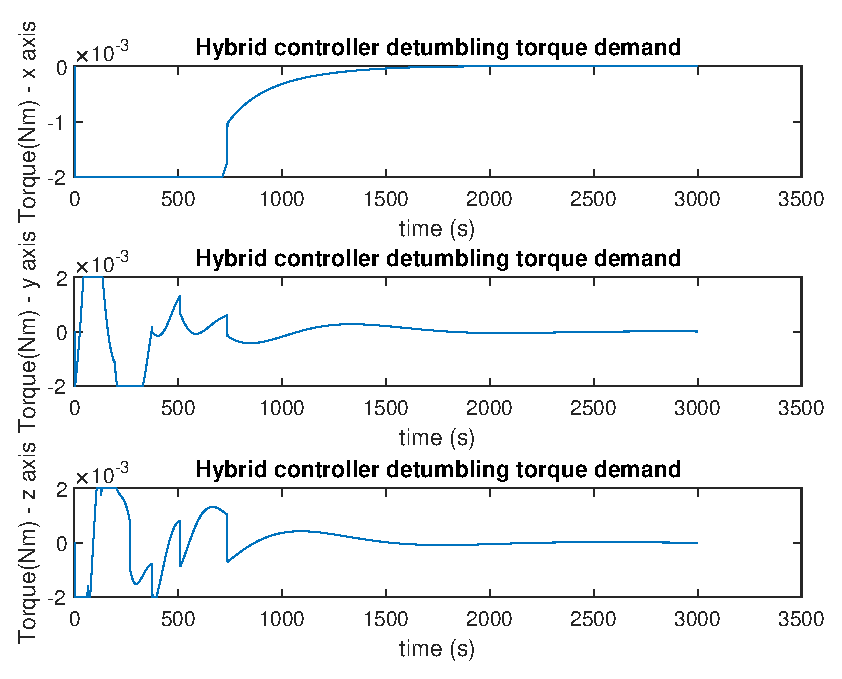
\includegraphics[width=0.7\linewidth]{figures/detumbling}
	\caption{Hybrid controller detumbling torque demand}
	\label{fig:detumbling}
\end{figure}

\begin{figure}[H]
	\centering
	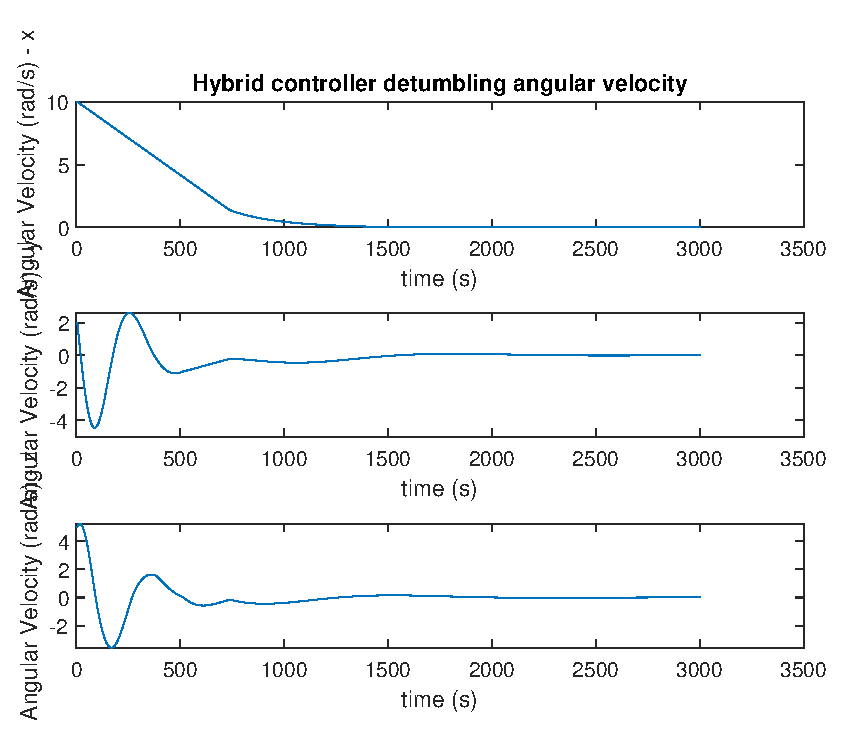
\includegraphics[width=0.7\linewidth]{figures/detumbling3}
	\caption{Hybrid controller detumbling angular velocity}
	\label{fig:omega}
\end{figure}



In the following chapter will be discussed shortly two attitude controller designs that are based on previous work \cite{PrevPro}. The two controllers calculate a torque demand that has to be produced from the motors. The first controller is based on the linearized model \eqref{eq:lele}, and thus is characterized as linear state feedback control, while the second one is based on the non-linear dynamics \eqref{eq:seom} creating a sliding manifold, a hyperplane, such that when the states are on the manifold, will converge to the desired reference. The non-linear controller is called Sliding Mode Control (SMC).\nomenclature[A]{\textbf{SMC}}{Sliding Mode Control}

\section{Linear controller} \label{sec:LC}

Since the norm of $ \vec{ {\bar{\omega}}} $ is known and equal to the orbital angular velocity ($\approx 0.0011$) comparing this value to $\frac{1}{2}$,becomes small, thus \eqref{eq:lele} can be simplified to 
\begin{flalign}
	\begin{bmatrix}
		\vec{ \dot {\tilde{q}}(t) } \\
		\vec{ \dot {\tilde{\omega}}(t) }
	\end{bmatrix} 	
	= 
	\begin{bmatrix}
		\underline{ 0}_{(3\times3)} &	\frac{1}{2} \underline{\vec 1}_{(3\times3)} \\
		\underline{ 0}_{(3\times3)} &	\underline{ 0}_{(3\times3)}
	\end{bmatrix} 
	\begin{bmatrix}
		\vec{  {\tilde{q}}(t) } \\
		{  {\tilde{\vec \omega}}(t) }
	\end{bmatrix} 	
	-
	\begin{bmatrix}
		\underline{\vec 0}_{(3\times3)} \\
		{\underline I_{s}^{-1}}
	\end{bmatrix} 	
	\vec {\tilde N_{ctrl}}
	\label{eq:lelele}
\end{flalign}
Three equal subsystems can be derived from \eqref{eq:lelele} as
\begin{flalign}
	\begin{bmatrix}
		\dot { \tilde {q_{i}}} \\
		\dot { \tilde { \omega_{i}}}
	\end{bmatrix} 	
	= 
	\begin{bmatrix}
		0&	\frac{1}{2}  \\
		0 &	 0
	\end{bmatrix} 
	\begin{bmatrix}
		\tilde{q_{i}}(t)  \\
		\tilde{\omega_{i}}(t) 
	\end{bmatrix} 	
	-
	\begin{bmatrix}
		0 \\
		I_{i,s}^{-1}
	\end{bmatrix} 	
	\tilde{N_{i}}
	\label{eq:subsys}
\end{flalign}
with $i = 1, 2, 3 $. The control torque was defined by the state feedback law as 
\begin{flalign}
	N_{i}	
	= 
	-
	\begin{bmatrix}
		k_{1} &	k_{2} 	
	\end{bmatrix} 
	\begin{bmatrix}
		\tilde{q_{i}}(t)  \\
		\tilde{\omega_{i}}(t) 
	\end{bmatrix} 	
	\label{eq:inputtorque}
\end{flalign}
leading to a second order closed loop system calculated as $det(s\underline{I} - (\underline{A} - \underline{BK}) )$. Identifying  this with a general second order equation $s^{2}+2\zeta\omega_{n}s+\omega_{n}^{2}$, with $\zeta$ be the dumping factor which was chosen to be equal to 1 leading to an over dumped response and $\omega_{n}$  the natural frequency $\omega_{n} =  \frac{2\pi}{60/0.35} $ with 60 be the value of the chosen rise time, the controller gains was derived as

\begin{flalign*}
	k_{1} = -2 I_{i,s} \omega_{n}^{2} 
	\label{eq:gainsl22}
\end{flalign*}
\begin{flalign*}
	k_{2} = -2\zeta I_{i,s} \omega_{n}^{2} 
	\label{eq:gainsl223}
\end{flalign*}
which give stability for the all values of $ \vec{ {\bar{\omega}}} $. 
\section{Sliding mode control} \label{sec:SM}

As described previously the sliding mode control scheme belongs to the class of non-linear control designs and is more robust compared to the linear, when disturbances are present. The objective of the SMC is the design, from a geometrical point of view, of a manifold in the state space which whenever the states are on the manifold, the behavior of the system will meet the specifications it is designed for, i.e convergence to the desired reference.  

\begin{figure}[H]
	\centering
	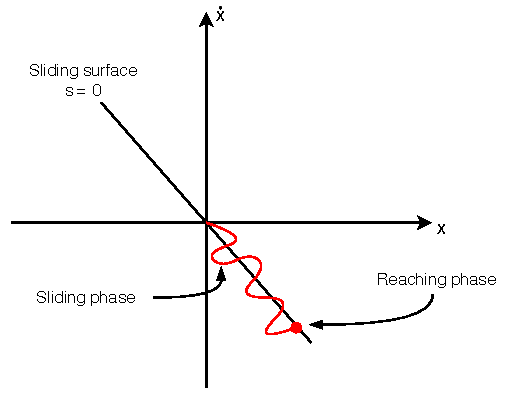
\includegraphics[width=0.5\linewidth]{figures/SM}
	\caption{Sliding mode behavior }
	\label{fig:SM}
\end{figure}

Introducing the small signal deviation of the states as
\begin{flalign}
	\vec{\tilde{q}} = \vec{  \bar{q}}^{-1} \otimes \vec{ q} 
	\label{eq:smallsignal22}
\end{flalign}
for the quaternion error and with $\vec{  \bar{q}}^{-1}$ be the reference quaternion and $\vec{ q} $ be the measured, and for the angular velocity
\begin{flalign}
	\vec{\tilde{\omega}}  = \vec{\omega}-\vec{\bar{\omega}}  
	\label{eq:smallsi4gnal4566}
\end{flalign}
with $\vec{\bar{\omega}}$ be the nominal value of the angular velocity. Moreover, by introducing the sliding variable as $s$ which depends on the error \nomenclature[S]{s}{Sliding variable} and is chosen to be 

\begin{flalign}
	s  = \underline{F}\vec{\tilde{q}} + \vec{\tilde{\omega}}  
	\label{eq:sliding variable}
\end{flalign}
with $\underline{F} = \alpha\ast diag[111]$ be a positive definite matrix. For $s=0$, $\vec{\tilde{\omega}} = - \alpha\ast\vec{\tilde{q}_{1:3}}$, where $\vec{\tilde{q}_{1:3}}$ denotes the vector part of the quaternion, and thus $\alpha$ can be designed appropriately, by trial and error to give the desired convergence for $\vec{\tilde{q}}$ meaning $[0;0;0;1]$, more details can be found in \todo{create appendix}.
The variable $s$ can be driven to 0 making use of a Lyapunov candidate function as
\begin{flalign}
	V  = \frac{1}{2} \vec{s}^{T}\vec{s} 
	\label{eq:sliding variable333}
\end{flalign} 
and in order to prove stability around $s=0$ a necessary condition is $\dot{V} < 0 $ for each $s\neq0$. The time derivative of \eqref{eq:sliding variable333} is written as
\begin{flalign}
	\dot{V}  = \frac{1}{2}( \dot{\vec{s}^{T}}\vec{s}+\vec{s}^{T}\dot{\vec{s}}) 
	\label{eq:sliding variable33333}
\end{flalign}
showing that $\vec{s}^{T}\dot{\vec{s}} < 0 $ $\forall s\neq0$ the condition may be satisfied.
Substituting \eqref{eq:sliding variable} is obtained
\begin{flalign}
	\dot{V}  = \vec{s}^{T} (\underline{F}{\vec{\dot{\tilde{q}}}} + {\vec{\dot{\tilde{\omega}}}}) 
	\label{eq:e33333}
\end{flalign}
and thus replacing \eqref{eq:seom} expressed for ${\vec{\dot{\tilde{\omega}}}}$ \eqref{eq:e33333} is written as 


\begin{flalign}
	\dot{V}  = \vec{s}^{T}\underline{I}_{s}^{-1}(-\underline{{\omega}}^\times\underline{I}_{s}\vec{\omega}-\underline{{\omega}}^\times\vec{h_{rw}}-\vec{N_{rw}}+\vec{N_{dis}} - \underline{I}_{s}\dot{\bar{\omega}} +\underline{I}_{s}\underline{F}{\vec{\dot{\tilde{q}}}} ) 
	\label{eq:444444}
\end{flalign}
by choosing the control as
\begin{flalign}
	\vec{N_{rw}}  = -\underline{{\omega}}^\times\underline{I}_{s}\vec{\omega}-\underline{{\omega}}^\times\vec{h_{rw}} - \underline{I}_{s}\dot{\omega} +\underline{I}_{s}\underline{F}{\vec{\dot{\tilde{q}}}}+\underline{I}_{s}\lambda sign(\vec{s})  ) 
	\label{eq:555555}
\end{flalign}

it can be seen in the above equations that the torque from the magnetorquers is not included since the magnetorquers are used only for desaturation.
\Eqref{eq:444444} can now be written as 
\begin{flalign}
	\dot{V} = -\vec{s}^{T}(-{\vec{\dot{\tilde{\omega}}}} +\lambda sign(\vec{s}) - \vec{N_{dis}}  )
	\label{eq:6666666}
\end{flalign}
consequently the condition $\dot{V} < 0 $ is satisfied if $\lambda >\rVert {\vec{\dot{\tilde{\omega}}}_{max}}\rVert +\rVert \vec{N_{dis}}\rVert$. The discontinuous function $sign$ is replace by the hyperbolic tangent function $tanh(\frac{\vec{s}}{\epsilon})$ in order to reduce the chattering around the manifold and $\epsilon$ is designed by trial and error.

